\documentclass{article}

\usepackage{graphicx}
\usepackage{tikz}
\usepackage{tikzsymbols}
\usetikzlibrary{calc,patterns,shapes.geometric}
\pagestyle{empty}
\usepackage[margin=0pt]{geometry}
\geometry{papersize={14in,12in}}

\def\centerarc[#1](#2)(#3:#4:#5){\draw[#1] ($(#2)+({#5*cos(#3)},{#5*sin(#3)})$) arc (#3:#4:#5);}

\begin{document}
	\begin{figure}
		\centering
		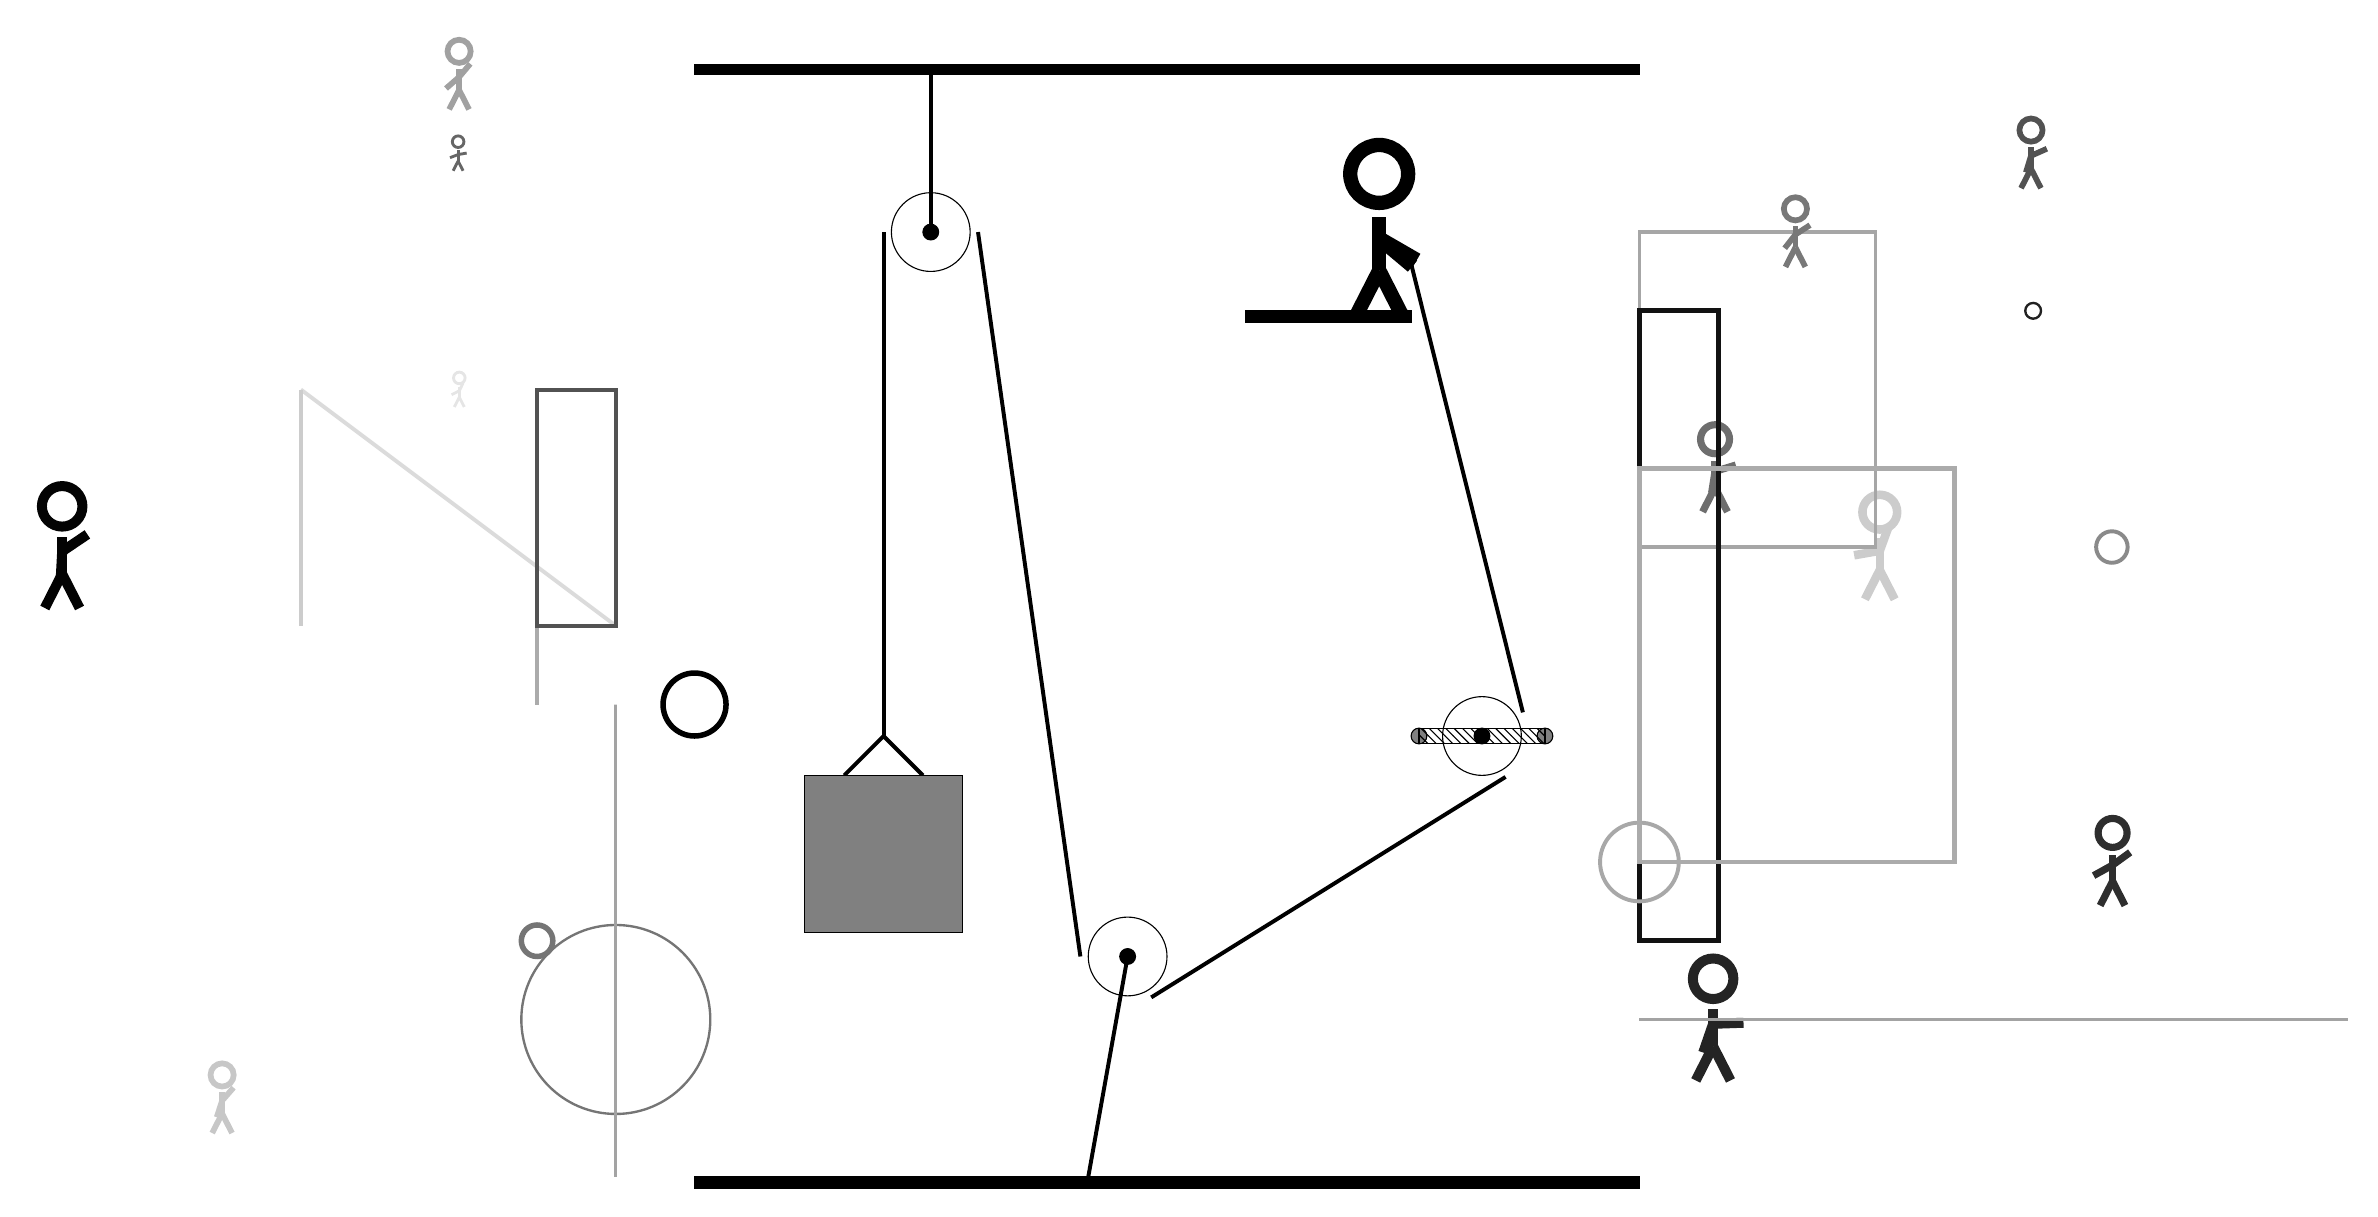
\begin{tikzpicture}
			%%%%% START %%%%%
			
			\draw[fill=black] (-2, 14) rectangle (10, 14.125);
			
			\draw (1, 12) circle (0.5);
			\draw[fill=black] (1, 12) circle (0.1);
			\draw[line width=0.5mm] (1, 14) -- (1, 12);
			
			\draw (3.5, 2.8) circle (0.5);
			\draw[fill=black] (3.5, 2.8) circle (0.1);
			\draw[line width=0.5mm] (3.5, 2.8) -- (3.0, 0);
			
			\draw[fill=white](8, 5.6) circle (0.5);
			\draw[fill=black] (8, 5.6) circle (0.1);
			\draw[fill=black!50] (8.8, 5.6) circle (0.1);
			\draw[fill=black!50] (7.2, 5.6) circle (0.1);
			\draw[pattern=north west lines, pattern color=black] (7.2, 5.7) rectangle (8.8, 5.5);
			
			\draw[line width=0.5mm](-0.1, 5.1) --  (0.4, 5.6) -- (0.9, 5.1);
			\draw[fill=black!50] (-0.6, 5.1) rectangle (1.4, 3.1);
			
			\draw[line width=0.5mm](0.4, 12) -- (0.4, 5.6);
			\centerarc[line width=0.5mm](1, 12)(180:0:0.6)
			\draw[line width=0.5mm](1.6, 12) -- (2.9, 2.8);
			\centerarc[line width=0.5mm](3.5, 2.8)(180:300:0.6);
			\draw[line width=0.5mm](3.8, 2.2804) -- (8.3, 5.0804);
			\centerarc[line width=0.5mm](8, 5.6)(300:390:0.6);
			\draw[line width=0.5mm](8.5196, 5.9) -- (7.05, 11.8);
			
			\node[line width=0.4mm, color=black!20] at (13, 8) {\Strichmaxerl[6][10][70]};
			
			\draw[line width=0.5mm, color=black!14](-7, 10) -- (-3, 7);
			\draw [line width=0.3mm, color=black!54](-3, 2) circle (1.2);
			\node[line width=0.7mm, color=black!82] at (16, 4) {\Strichmaxerl[5][29][36]};
			
			\node[line width=0.5mm, color=black!10] at (-5, 10) {\Strichmaxerl[2][27][64]};
			\node[line width=0.4mm, color=black!86] at (11, 2) {\Strichmaxerl[7][71][2]};
			
			\draw[line width=0.4mm, color=black!35] (10, 12) rectangle (13, 8);
			
			\node[line width=0.4mm, color=black!37] at (-5, 14) {\Strichmaxerl[4][41][50]};
			\node[line width=0.3mm, color=black!68] at (15, 13) {\Strichmaxerl[4][73][24]};
			
			\draw[line width=0.4mm, color=black!36] (-3, 0) rectangle (-3, 6);
			\node[line width=0.4mm, color=black!99] at (-10, 8) {\Strichmaxerl[7][87][34]};
			
			\draw [line width=0.3mm, color=black!87](15, 11) circle (0.1);
			\draw [line width=0.5mm, color=black!46](16, 8) circle (0.2);
			\node[line width=0.4mm, color=black!53] at (12, 12) {\Strichmaxerl[4][52][33]};
			\node[line width=0.3mm, color=black!57] at (11, 9) {\Strichmaxerl[5][81][17]};
			\draw [line width=0.7mm, color=black!100](-2, 6) circle (0.4);
			
			\draw[line width=0.5mm, color=black!20](-7, 7) -- (-7, 10);
			
			\draw[line width=0.5mm, color=black!36](10, 2) -- (19, 2);
			\node[line width=0.7mm, color=black!60] at (-5, 13) {\Strichmaxerl[2][21][10]};
			
			\draw[line width=0.6mm, color=black!93] (10, 11) rectangle (11, 3);
			\draw [line width=0.5mm, color=black!34](10, 4) circle (0.5);
			
			\draw[line width=0.5mm, color=black!33](-4, 9) -- (-4, 6);
			\draw[line width=0.5mm, color=black!68] (-3, 10) rectangle (-4, 7);
			\draw[line width=0.6mm, color=black!33] (10, 4) rectangle (14, 9);
			\node[line width=0.4mm, color=black!22] at (-8, 1) {\Strichmaxerl[4][72][49]};
			
			\draw [line width=0.7mm, color=black!54](-4, 3) circle (0.2);
			
			
			\node at (6.75, 12) {\Strichmaxerl[10][-220][-30]};
			\draw[fill=black] (5, 11) rectangle (7.1, 10.85);
			
			\draw[fill=black] (-2, 0) rectangle (10, -0.15);
			
			%%%%% END %%%%%
		\end{tikzpicture}
	\end{figure}	
\end{document}